\section{Formalizing Instantaneous Reactors}
\label{section:formal-inst-reactors}

Despite the Simple Reactor model being relatively small, formalizing it and especially proving properties about it, is an extensive undertaking.
To achieve a clean separation of concerns, we split the implementation into two parts:

\begin{itemize}
    \item In this section we implement the instantaneous components of the model, i.e. everything that does not involve time.
    We call this subset the \emph{Instantaneous Reactor} model.
    In Section \ref{section:determinism} we prove determinism only for the Instantaneous Reactor model.
    \item In Section \ref{section:time} we add the time-based aspects of the Simple Reactor model as a generalization of the Instantaneous Reactor model.
    That is, we add them \emph{on top} and do not make any changes to the Instantaneous Reactor model in the process.
\end{itemize}

\subsection{Primitives}

One issue in the Simple Reactor model is circular definitions. 
To avoid this in our formalization, it is important to be clear about which primitives are used by other objects in their definitions.
For example, if ports are a component of reactors, and reactions also reference ports in their definition, then having reactions as a part of reactors makes the definitions circular.
Hence, we first define some primitives that are used by other objects.

Values ($\in \mathfrak{V}$) are supposed to be opaque, but have one requirement: they should have a notion of equality.
To achieve this, we don't define a type of values explicitly, but instead make all other definitions dependent on some type parameter \lstinline{υ}.
That way, it is impossible for any definitions that use \lstinline{υ} to depend on \emph{concrete} instances of \lstinline{υ} --- i.e. the values are opaque.
We ensure that this type is equatable, by constraining it to the type class \lstinline{decidable_eq}:

\begin{lstlisting}
variables (υ : Type*) [decidable_eq υ]
\end{lstlisting}

\noindent We can model a reactor's ports and state variables as lists over such values.
Using names like \lstinline{reactor.ports} is part of Lean's namespace syntax. 
Here we declare that the definitions of \lstinline{ports} and \lstinline{state_vars} are part of the namespace \lstinline{reactor}:

\begin{lstlisting}
def reactor.ports := list (option υ)
def reactor.state_vars := list υ
\end{lstlisting}

\noindent We account for the absent value $\epsilon$, by using optional values.
Wrapping any type in the \lstinline{option} type makes the values optional, by adding a \lstinline{none} value, which is generally used to represent the absence of a value.
We assume here that $\epsilon$ is only intended for modeling absence of values in \emph{ports}, and hence omit the optionality for state variables.
The term \emph{port assignment} is used throughout this thesis to mean \emph{an instance of \lstinline{reactor.ports υ}}.
As an example of a port assignment, consider the following instance:

\begin{lstlisting}
def p : reactor.ports υ := [some 1, none, some 2, some 1]
\end{lstlisting}

\noindent If \lstinline{p} are the input ports of some reactor, then that reactor has exactly four input ports, where the value in the second port is absent.

Using lists for these components solves some inaccuracies of the Simple Reactor model. 
Firstly, we now know where their values live: in the lists. 
Secondly, we get the type of their identifiers for free, as we can just use the lists' indices ($\in \mathbb{N}$) as IDs.
Since a reactor will hold two instances of \lstinline{reactor.ports}, one for its inputs and one for its outputs, these IDs will in fact be ambiguous within a reactor.
That is, an arbitrary port-ID \verb|n| could refer either to the \verb|n|th input port or the \verb|n|th output port. 
This ambiguity will always be resolved by context.

It should be noted here that the length of these lists is not fixed, so we could change the number of a reactor's ports, by changing the number of elements in one of these lists.
This can be avoided, by instead using a fixed-length vector type.
The downside is that this leads to dependent type hell, so we opt for the GIGO-approach here by declaring that port assignments' length should not be changed during execution.

\vspace{3mm}

\noindent Many of the definitions of reactor components in this thesis are accompanied by auxiliary definitions.
For example, we explicitly define fully absent \lstinline{ports} and a related proposition:

\begin{lstlisting} 
def ports.empty (n : ℕ) : ports υ := list.repeat none n
def is_empty (p : ports υ) : Prop := (p = ports.empty υ p.length)
\end{lstlisting}

\noindent Definitions like these improve the comprehensibility of later definitions greatly.
We will sometimes use such definitions without showing them, and instead resort to describing their functionality in prose. 

\subsection{Reactors \& Reactions}

Using \lstinline{ports} and \lstinline{state_vars} makes the definition of reactors straightforward:

\begin{lstlisting}
structure reactor :=
  (input : ports υ)
  (output : ports υ)
  (state : state_vars υ)
  (priorities : finset ℕ)
  (reactions : ℕ → reaction υ)
\end{lstlisting}

\noindent The notable fields are \lstinline{priorities} and \lstinline{reactions}.
One of the issues with the definition of reactors in the Simple Reactor model is that since the reactions ($\mathcal{N}$) are in a set, they all have to be unique.
Additionally, to ensure that no two reactions have the same priority, the priority function ($P$) has to be injective.
We can circumvent both of these problems, by switching the positions of priorities and reactions.
That is, what was the set of \emph{reactions} becomes the set of \emph{priorities}, and the priority function becomes a reaction function, which maps the priorities to concrete reactions.
Thus, we use a reaction's priority as an identifier for it.
To avoid dependent type hell, we \emph{don't} restrict the domain of the \lstinline{reactions} function to be \emph{exactly} the reactor's set of priorities.
Instead, we require a function from \emph{all} \lstinline{ℕ}, but only ever employ the map for \lstinline{n : ℕ} which are in the set of priorities.

Alternatively, we could use a partial function \lstinline{ℕ → option (reaction υ)} and add a constraint that all \lstinline{n ∈ priorities} must map to a non-\lstinline{none} value.
This causes inconvenience at the call-site though, as we have to unwrap the optional values.    

\vspace{3mm}

\noindent This definition of \lstinline{reactor} is only valid, if we've already defined \lstinline{reaction}.
That is, our definition of \lstinline{reaction} cannot depend on \lstinline{reactor}:

\begin{lstlisting}
structure reaction :=
  (dᵢ : finset ℕ) 
  (dₒ : finset ℕ)
  (triggers : finset {i // i ∈ dᵢ})
  (body : ports υ → state_vars υ → ports υ × state_vars υ)
  (in_con : ∀ {i i'} s, (i =dᵢ= i') → body i s = body i' s)
  (out_con : ∀ i s {o}, o ∉ dₒ → (body i s).1.nth o = none) 
\end{lstlisting}

\noindent The sets \lstinline{dᵢ} and \lstinline{dₒ} are the reaction's dependencies and antidependencies ($D$ and $D^\vee$).
Throughout this thesis we also refer to them as \emph{input-} and \emph{output-dependencies}.
They contain IDs of their enclosing reactor's ports, i.e. indices into the reactor's \lstinline{input} and \lstinline{output} lists.
The \lstinline{triggers} are a subset of \lstinline{dᵢ}, defined as a set that contains instances of the subtype \lstinline|{i // i ∈ dᵢ}|.

The first substantial change relative to the Simple Reactor model is made to a reaction's body ($B$).
Our original definition declared it to be opaque code, which we have determined to be problematic.
Here we define it as a \emph{function} that maps from an input-port assignment and state variables to an output-port assignment and new state.
We define the function in curried form, as this makes the call-site cleaner and easily allows partial application.\footnote{
  It is canonical to define functions in this form in Lean.
}
The symbol \lstinline{×} in the target type is syntactic sugar for the \lstinline{prod} type.

When we run a reaction as part of a reactor\footnote{Cf. Section \ref{section:execution-model}.}, its body receives the reactor's input-ports and state variables as inputs, and the body's outputs are incorporated into the reactor by a dedicated function.
The \lstinline{body} function has the option of not writing to an output-port, by returning the absent value for the specific port.
That is, the returned instance of \lstinline{ports υ} holds a value of \lstinline{none} at the corresponding index.

To ensure that this definition of \lstinline{body} behaves in a way that is analogous to that of the Simple Reactor model, we need to enforce some restrictions:

\begin{enumerate}
    \item A \lstinline{body}'s outputs can only depend on \emph{those} ports which are part of its input-dependencies \lstinline{dᵢ}.
    Thus, we achieve the same behavior as if we were to restrict the domain of the function to be exactly \lstinline{dᵢ}. 
    This restriction is enforced by the property \lstinline{in_con}:
    Given two input-port assignments \lstinline{i} and \lstinline{i'} that have the same values for all ports in \lstinline{dᵢ} (written as \lstinline{i =dᵢ= i'}), the output of \lstinline{body} has to be the same.
    For the purposes of this thesis, parameters that are enclosed by braces (here \lstinline|{i i'}|) can be considered to be the same as parameters enclosed by parentheses.
    \item A reaction should only be able to write to \emph{those} ports which are part of its output-dependencies \lstinline{dₒ}.
    Hence, the output-port assignment returned by \lstinline{body} should be \lstinline{none} for all ports that are not in \lstinline{dₒ}.
    This is enforced by \lstinline{out_con}:
    Given any inputs (\lstinline{i} and \lstinline{s}) and an output-port ID \lstinline{o} which is not in \lstinline{dₒ}, running the body must yield a value of \lstinline{none} for \lstinline{o}.
    The expression \lstinline{(body i s).1.nth o = none} expresses precisely this last proposition.
\end{enumerate}

\subsection{Reactor Networks}

As mentioned in Section \ref{section:simpel-reactors}, the Simple Reactor model has no notion of nested reactors.
Instead, we build reactor networks using a global graph structure.
We have previously laid the foundations for this by defining \lstinline{lgraph}.\footnote{Cf. Section \ref{section:hell}.}
To construct a reactor network from an L-graph, we need to define which types the graph's \emph{identifiers} and \emph{edges} should have.

\paragraph{Identifiers:}

In \lstinline{reactor} and \lstinline{reaction} we used instances of \lstinline{ℕ} for identifying reactions and ports.
This works great as long as we only have \emph{one} reactor.
In a reactor \emph{network}, we need to extend these IDs to also specify the reactor they live in:

\begin{lstlisting}
def reactor.id := ℕ

structure reaction.id := 
  (rtr : reactor.id) 
  (rcn : ℕ)

structure port.id := 
  (rtr : reactor.id) 
  (prt : ℕ)
\end{lstlisting}

\noindent That is, every reactor in a network has a unique number ($\in \mathbb{N}$) associated with it.
Reactions and ports can then be globally identified by a combination of their reactor and local ID.

\paragraph{Edges:}

While the vertices in a reactor network are reactors, the components that should be connected by edges are their \emph{ports}.
Hence, we need the edges in a reactor network to have a concept of which ports they are connecting:

\begin{lstlisting}
structure inst.network.graph.edge :=
  (src : port.id)
  (dst : port.id)
\end{lstlisting}

\noindent We don't distinguish between types for input-port and output-port IDs, since we know that the \lstinline{src} always refers to an output-port and the \lstinline{dst} to an input-port.

\paragraph{Graph:}

An \lstinline{inst.network.graph} is now just an \lstinline{lgraph}, that uses \lstinline{reactor.id} as its ID-type, \lstinline{reactor υ} as its data-type and \lstinline{inst.network.graph.edge} as its edge-type:

\begin{lstlisting}
def inst.network.graph : Type* := 
  lgraph reactor.id (reactor υ) inst.network.graph.edge
\end{lstlisting}

\noindent For convenience, we define some accessors on this structure:

\begin{lstlisting}
def rtr (η : inst.network.graph υ) (i : reactor.id) : reactor υ 
  := η.data i

def rcn (η : inst.network.graph υ) (i : reaction.id) : reaction υ 
  := (η.rtr i.rtr).reactions i.rcn
\end{lstlisting}

\paragraph{Network:}

While this concrete graph \emph{structure} is well-suited for our purposes, it is not sufficiently restrictive.
There are two issues that need to be addressed:

\begin{enumerate}
  \item It is currently possible to have multiple edges ending in the same port.
  This is explicitly forbidden in the Reactor model.
  As long as we don't define a global order on reactors (as we have with reactions in a reactor), this restriction is necessary for maintaining determinism during value propagation.
  \item Ports can be connected in such a way that associated reactions can have cyclic precedence.
  In Section \ref{section:execution-model-steps} we stated that execution is only defined for networks with acyclic precedence graphs.
  Here we disallow precedence-cyclic networks entirely.
\end{enumerate}

\noindent Hence, our previous definition only defined a network \emph{graph}.
The definition of a complete instantaneous reactor network wraps such an \lstinline{inst.network.graph}, and requires additional proofs about it:

\begin{lstlisting}
structure inst.network :=
  (η : inst.network.graph υ)
  (unique_ins : η.has_unique_port_ins) -- addresses Issue 1
  (prec_acyclic : η.is_prec_acyclic)   -- addresses Issue 2
\end{lstlisting}

\noindent The first restriction is easy to implement.
We require that all (non-equal) edges in the network have different destinations:

\begin{lstlisting}
def has_unique_port_ins (η : inst.network.graph υ) : Prop :=
  ∀ (e ∈ η.edges) (e' ∈ η.edges), e ≠ e' → e.dst ≠ e'.dst
\end{lstlisting}

\noindent To implement the second restriction, we first need to formalize a notion of \emph{precedence} in a reactor network.

\break

\subsection{Precedence Graphs}

The intuition behind precedence in a reactor network is rather simple. 
A reaction $r$ can take precedence over another reaction $s$ if it satisfies at least one of the following conditions:

\begin{enumerate}
  \item $r$ and $s$ live in the same reactor, and $r$ has a higher priority than $s$.
  \item A dependency of $s$ is connected to an antidependency of $r$.\footnote{
    $r$ and $s$ may or may not live in the same reactor.
  }
  \item $r$ is transitively determined to take precedence over $s$. 
\end{enumerate}

\noindent While the first condition can be analyzed locally, the latter require a global view of dependencies.
Hence, we define a \emph{precendence graph}.
A precedence graph connects \emph{reactions}, such that the edges represent their immediate (non-transitive) precedences:

\begin{lstlisting}
structure prec.graph.edge := 
  (src : reaction.id)
  (dst : reaction.id)

def prec.graph : Type* := 
  lgraph reaction.id (reaction υ) prec.graph.edge
\end{lstlisting}

\noindent Again, while this concrete graph \emph{structure} is well-suited for our purposes, it is not sufficiently restrictive.
We need a way of ensuring that its vertices and edges actually reflect the precedences for a given network graph.
If this is the case, we call the precedence graph \emph{well-formed} over a fixed instantaneous network graph:

\lstset{numbers=left, xleftmargin=1.5em}
\begin{lstlisting}
def is_well_formed_over 
  (ρ : prec.graph υ) (η : inst.network.graph υ) : Prop :=
    ρ.edges_are_well_formed_over η ∧
    ρ.ids_are_well_formed_over   η ∧ 
    ρ.data_is_well_formed_over   η  
\end{lstlisting}

\noindent The three expression (Lines 3-5) are propositions about the three components of \lstinline{lgraph}, and therefore \lstinline{prec.graph}: edges, IDs and data.

\paragraph{Edges:}

The first property (Line 3) is the most interesting.
It makes sure that the precedence graph contains edges between exactly those reactions that satisfy precedence conditions 1 or 2:

\begin{lstlisting}
def edges_are_well_formed_over 
  (ρ : prec.graph υ) (η : inst,network.graph υ) : Prop :=
    ∀ e : edge, e ∈ ρ.edges ↔ 
      internally_dependent e.src e.dst ∨
      externally_dependent e.src e.dst η
\end{lstlisting}

\noindent Lines 4 and 5 correspond to precedence conditions 1 and 2 respectively, and are not further explored here.

\paragraph{Identifiers:}

\noindent The second property in \lstinline{is_well_formed_over} (Line 4), expresses the restriction that a precedence graph must contain exactly those reactions (represented by their IDs) which are present in the network graph:

\begin{lstlisting}
def ids_are_well_formed_over 
  (ρ : prec.graph υ) (η : inst.network.graph υ) : Prop :=
    ∀ i : reaction.id, i ∈ ρ.ids ↔ 
      i.rtr ∈ η.ids ∧ 
      i.rcn ∈ (η.rtr i.rtr).priorities
\end{lstlisting}
\lstset{numbers=none, xleftmargin=0em}

\noindent Recall here that a reactor identifies its reactions by their priorities. 
Hence, Line 5 states that \lstinline{i.rcn} should be a member of the reactor identified by \lstinline{i.rtr}.

\paragraph{Data:}

We consider a precedence graph's \emph{data} to be well-formed over a given instantaneous network graph $\eta$, if it corresponds exactly to the reactions in $\eta$.
That is, the reaction-IDs in \lstinline{ρ} have to map to the same reactions as in \lstinline{η}.
Hence, we explicitly ignore the \emph{values} in the network graph, since they do not affect precedence.

\begin{lstlisting}
def data_is_well_formed_over 
  (ρ : prec.graph υ) (η : inst.network.graph υ) : Prop :=
    ∀ i : reaction.id, ρ.rcn i = η.rcn i
\end{lstlisting}

\noindent Thus, a precedence graph that is well-formed over a network graph \lstinline{η} contains precisely all reactions present in \lstinline{η}, while connecting exactly those reactions by edges that fulfill precedence conditions 1 or 2.

\paragraph{Transitivity:}

To find \emph{transitive} precedences between reactions (precedence condition 3), we need to further analyze the precedence graph.
Namely, if the precedence graph has a \emph{path} from one reaction to another, then the former takes precedence over the latter.
The notion of paths is defined directly on \lstinline{lgraph}. 
If \lstinline{r} and \lstinline{s} are IDs and \lstinline{ρ} is an L-graph, then the notation \lstinline{r~ρ~>s} is used for the proposition that there is a path from \lstinline{r} to \lstinline{s} in \lstinline{ρ}.
By using paths to express transitive precedence, we can define the \lstinline{is_prec_acyclic} property, required for \lstinline{inst.network}:

\begin{lstlisting}
def lgraph.is_acyclic (g : lgraph ι δ ε) : Prop := 
  ∀ i, ¬(i~g~>i)

def inst.network.graph.is_prec_acyclic 
  (η : inst.network.graph υ) : Prop :=
    ∀ ρ : prec.graph υ, (ρ ⋈ η) → ρ.is_acyclic
\end{lstlisting}

\noindent The notation \lstinline{(ρ ⋈ η)} stands for \lstinline{(ρ.is_well_formed_over η)}.
Thus, we require all well-formed precedence graphs over \lstinline{η} to be acyclic.

\subsection{Execution Model}
\label{section:execution-model}

Now that we have a formal notion of instantaneous reactor networks, we can define what it means to \emph{run} them.
For this we use a hierarchy of small algorithms, composed into a singular \lstinline{run} function.

\subsubsection{Outline}

Two of the algorithms required for the \lstinline{run} function are special, in that we do not define them explicitly.
Instead, we define their behavior by constraints.

\lstset{numbers=left, xleftmargin=1.5em}
\begin{lstlisting}
structure prec_func :=
  (func : inst.network υ → prec.graph υ)
  (well_formed : ∀ σ, (func σ) ⋈ σ.η)

structure topo_func :=
  (func : prec.graph υ → list reaction.id)
  (is_topo : ...)
\end{lstlisting}
\lstset{numbers=none, xleftmargin=0em}

\noindent An instance of \lstinline{prec_func} is a function that generates the precedence graph for a given network (Line 2), while being subject to the constraint that it must produce only well-formed precedence graphs (Line 3).
We don't define this function explicitly, as it is of no interest to our model \emph{how} the function works.
All we care about is \emph{what} it returns.
The same holds for instances of \lstinline{topo_func}.
All we need to know about such a function is that it can compute a topological ordering for a precedence graph.\footnote{
  The \lstinline{is_topo} property (Line 7) constrains the output of \lstinline{func} to be a topological ordering.
  The exact implementation is omitted here to hide unnecessary detail. 
}
It is irrelevant \emph{how} it does it.

This aspect of the execution model is not simply a convenience, but rather a feature of the Reactor model.
The execution of reactor networks behaves the same, independently of the concrete precedence and topological-ordering functions.
Thus, formalizing \lstinline{prec_func} and \lstinline{topo_func} in this way, ensures that we retain this property of independence.\footnote{
  A proof of independence will be covered in Section \ref{section:indep}.
}

\vspace{3mm}

\noindent The \emph{explicitly} defined algorithms required to define instantaneous reactor network execution align quite closely with the following steps.
They can be thought of as a more rigorous version of the steps presented in Section \ref{section:execution-model-steps}, while omitting time-based aspects like the global tag, event queue and actions.

\begin{enumerate}
  \item Generate the reaction queue as a topological ordering over the network's precedence graph.
  This is covered by \lstinline{prec_func} and \lstinline{topo_func}.
  \item For each reaction in the reaction queue, execute it.
  \begin{enumerate}
    \item Compute the reactor that we get by running the reaction, isolated to its reactor (without any value propagation).
    \item Apply that modified reactor to the reactor network.
    \begin{enumerate}
      \item Swap the ``old'' reactor for the new one, i.e. point the relevant reactor-ID to the new reactor created in step (a).
      \item Propagate the values of all of the output-ports that were written to by the executed reaction.
    \end{enumerate}
  \end{enumerate}
\end{enumerate}

\begin{figure}[h]
\centering
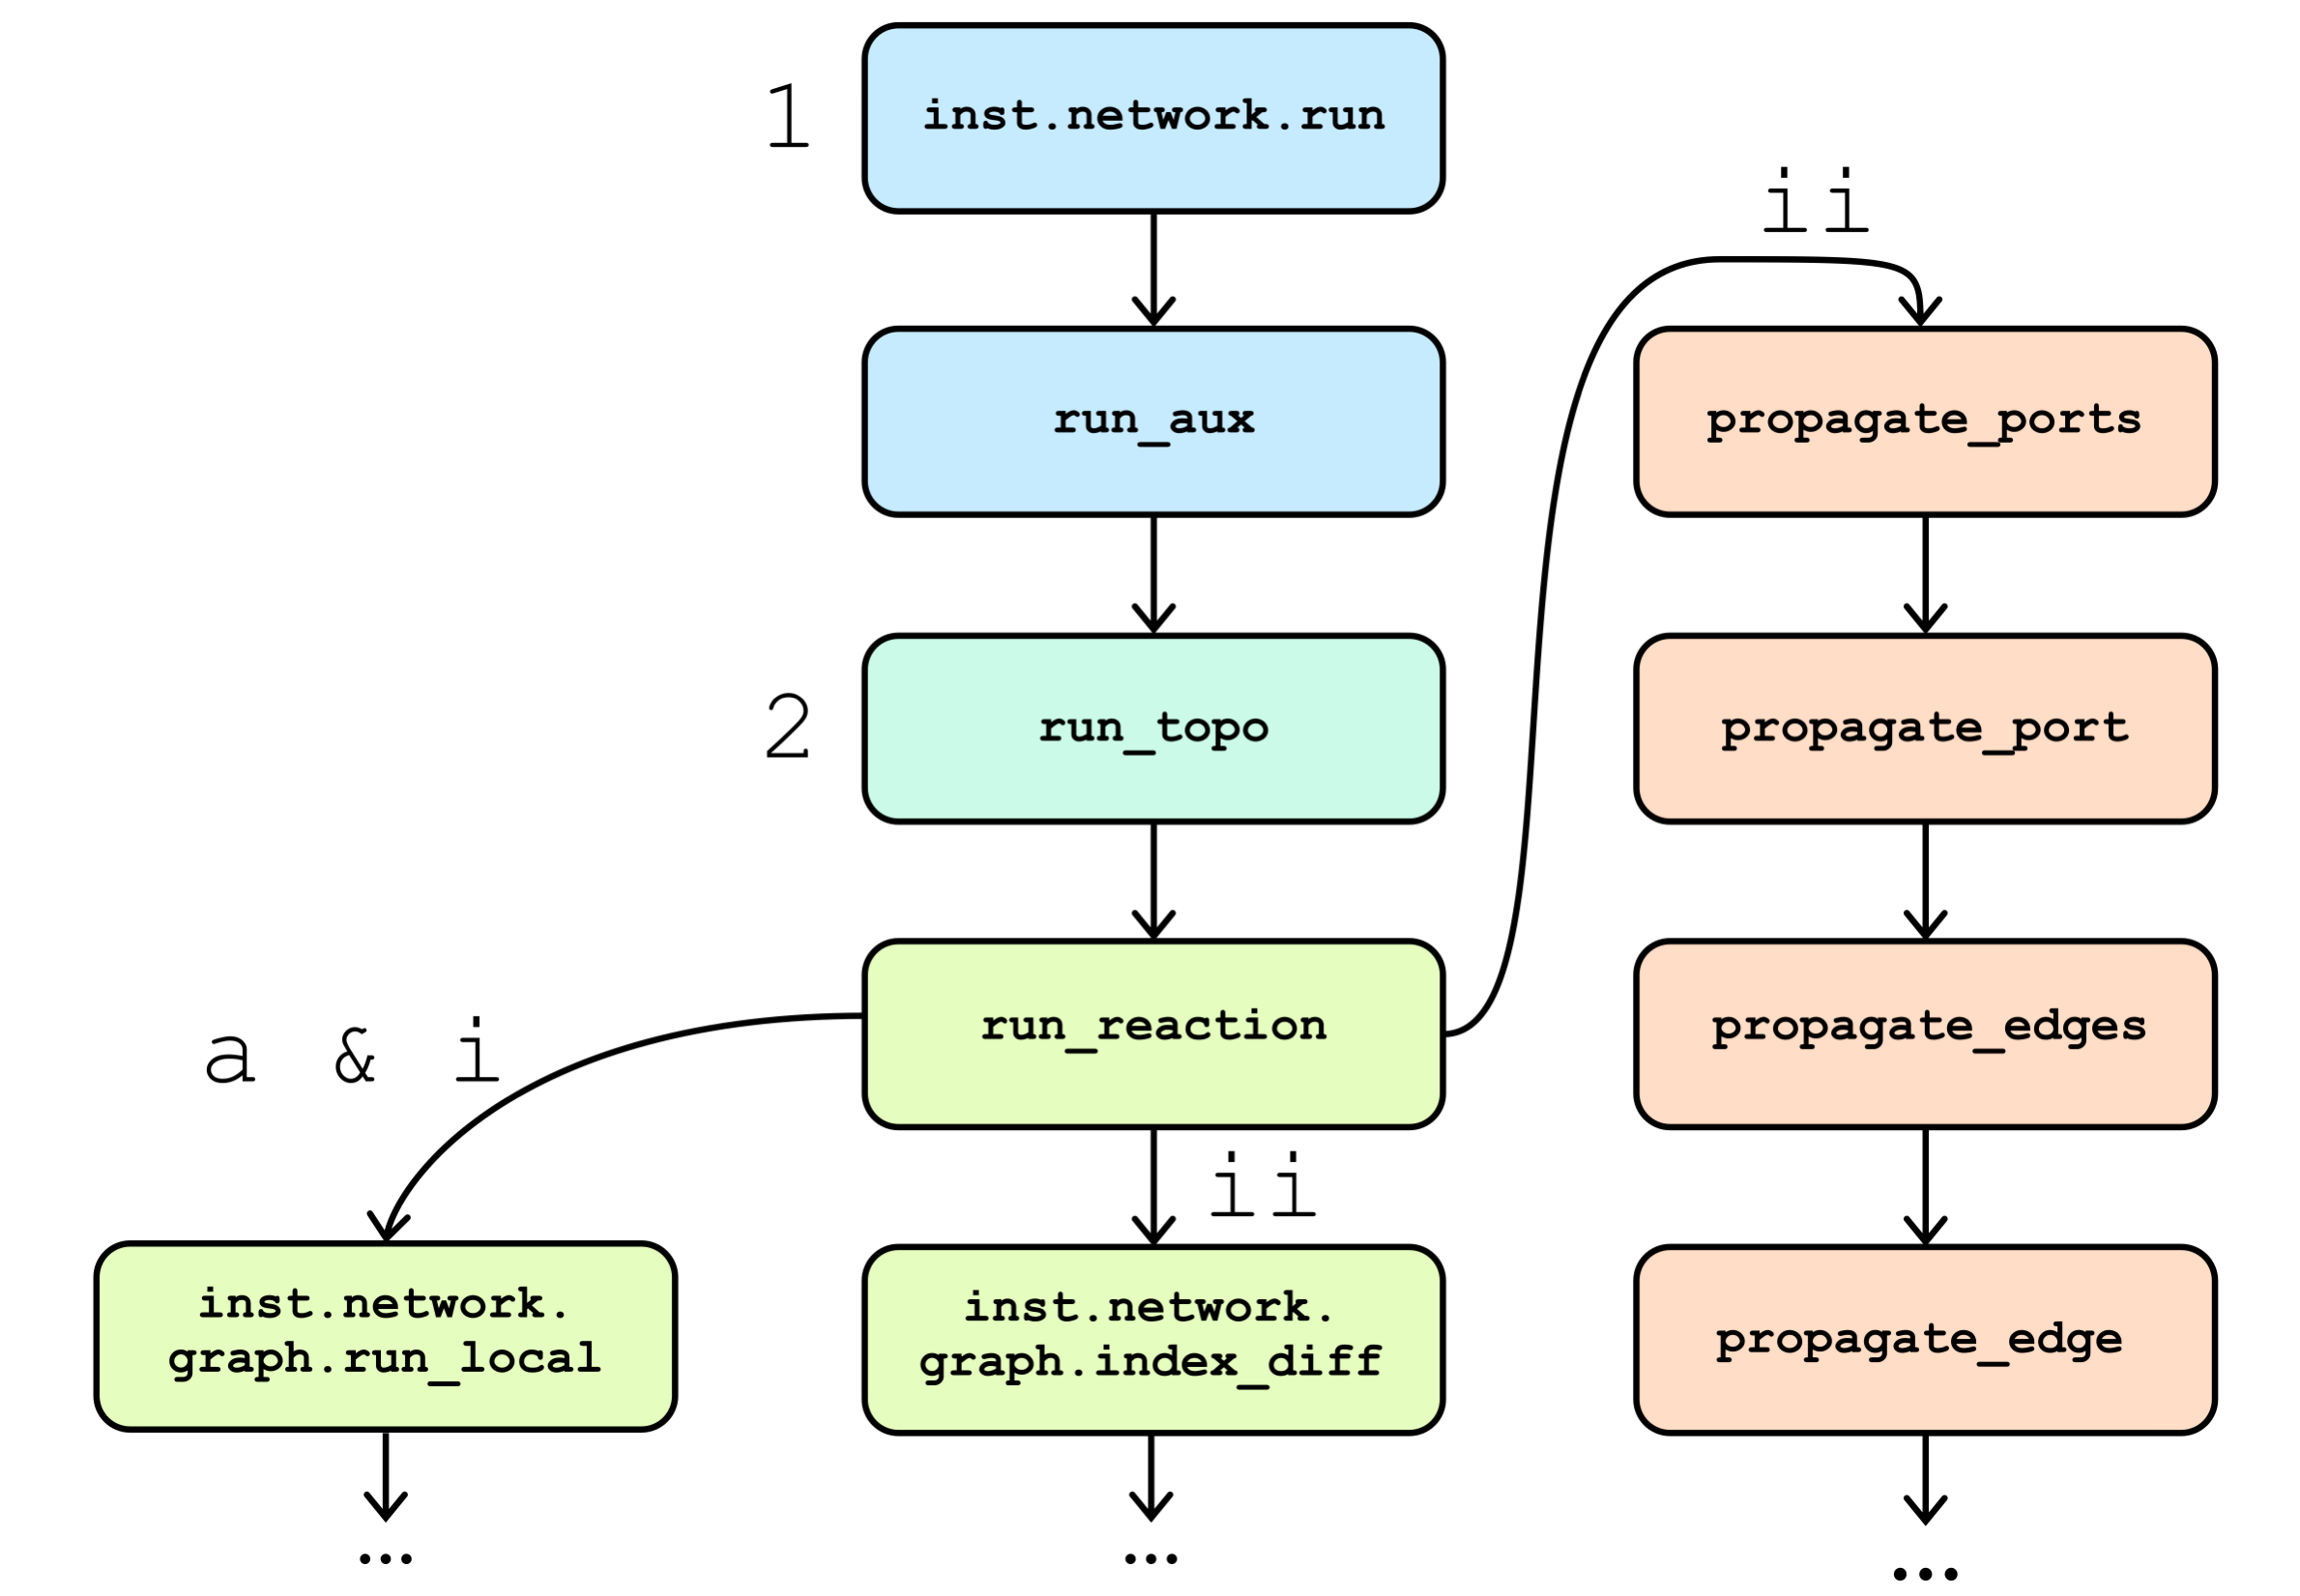
\includegraphics[width=\columnwidth]{run-func}
\caption{Explicit algorithms for instantaneous reactor network execution}
\label{fig:exec-plan}
\end{figure}

\noindent Figure \ref{fig:exec-plan} shows that some of these steps are themselves subdivided in the implementation.
This is especially true for value propagation.

\subsubsection{Implementation}

Algorithms in Lean are fundamentally functional (as opposed to imperative).
That is, they cannot contain \emph{sequences} of statements.
Instead, an algorithm consists of one, possibly deeply nested, expression which computes the desired result.
For the Instantaneous Reactor model, the \lstinline{run} function is the root expression which computes the result of running a given reactor network:

\begin{lstlisting}
def run 
  (σ : inst.network υ) (fₚ : prec_func υ) (fₜ : topo_func υ) : 
  inst.network υ :=
    run_aux σ (fₜ (fₚ σ))
\end{lstlisting}

\noindent This definition exemplifies the structure that most of the following algorithms have.
They compute one small partial result and pass it on to the next algorithm (according to Figure \ref{fig:exec-plan}).
In the case of \lstinline{run}, we only compute a topological ordering (\lstinline{fₜ (fₚ n)}) for the given network, and pass it to \lstinline{run_aux}:

\begin{lstlisting}
def run_aux (σ : inst.network υ) (t : list reaction.id) : 
  inst.network υ :=
    { inst.network . η := σ.η.run_topo t, 
      unique_ins := ..., prec_acyclic := ... }
\end{lstlisting}

\noindent The syntax \lstinline|{ inst.network . η := ..., ... }| is a constructor for structures.
In Lean, appending \lstinline{_aux} to a function's name is common practice, when a function needs to be divided into multiple parts that are tightly coupled.
In the case of \lstinline{run_aux}, all we do is forward the reaction queue from \lstinline{run} to \lstinline{run_topo}, which computes the result of executing that reaction queue on the network's graph.
The main function of \lstinline{run_aux} is to then reassemble that result back into an instance of \lstinline{inst.network}, by providing proofs that it still fulfills the \lstinline{unique_ins} and \lstinline{prec_acyclic} properties.\footnote{
  Cf. Section \ref{section:equiv}.
}

\vspace{3mm}

\noindent The \lstinline{run_topo} function iterates over the given reaction queue, executes each reaction and combines the outputs into a single result.
For this it uses a \emph{fold}, as is typical in functional languages:

\begin{lstlisting}
def run_topo (η : inst.network.graph υ) (t : list reaction.id) : 
  inst.network.graph υ := 
    t.foldl run_reaction η
\end{lstlisting}

\noindent The way in which this function executes each reaction, is by calling \lstinline{run_reaction}:

\begin{lstlisting}
def run_reaction (η : inst.network.graph υ) (i : reaction.id) : 
  inst.network.graph υ :=
    (η.run_local i).propagate_ports 
    ((η.run_local i).index_diff η i.rtr role.output).val.to_list
\end{lstlisting}

\noindent This function is central to our implementation. It performs three steps:

\begin{enumerate}
  \item It runs the given reaction in its reactor and swaps the ``old'' reactor for the executed one in the network graph: \lstinline{(η.run_local i)}.
  Running a reaction isolated in its reactor has its own set of steps, which we omit here for brevity.
  \item It computes which output-ports have been written to as a result of the reaction's execution (\lstinline{index_diff}).
  \item It propagates the values of the affected ports according to the network graph's connections (\lstinline{propagate_ports}).
\end{enumerate}

\paragraph{Output Propagation:}

Output propagation has an entire hierarchy of sub-steps of its own.
For the sake of brevity, we show them all at once.
The following definitions live in the \lstinline{inst.network} namespace.
Thus, any type whose name starts with ``\lstinline{graph}'' actually starts with ``\lstinline{inst.network.graph}''.

\lstset{numbers=left, xleftmargin=2em}
\begin{lstlisting}
def propagate_ports (η : graph υ) (ps : list port.id) : 
  graph υ :=
    ps.foldl propagate_port η

def propagate_port (η : graph υ) (p : port.id) : 
  graph υ := 
    η.propagate_edges (η.eₒ p).val.to_list 

def propagate_edges (η : graph υ) (es : list graph.edge) : 
  graph υ := 
    es.foldl propagate_edge η

def propagate_edge (η : graph υ) (e : graph.edge) : 
  graph υ := 
    η.update_port role.input e.dst (η.port role.output e.src)
\end{lstlisting}
\lstset{numbers=none, xleftmargin=0em}

\noindent Value propagation is highly repetitive. 
These functions specify that propagation of a list of ports requires repeated propagation of a single port (Line 3).
Propagation of a single port requires propagation of all of its connected edges (Line 7), and propagation of a list of edges requires repeated propagation of a single edge (Line 11).
The non-trivial expressions contained in this are:

\begin{itemize}
  \item Line 7:
  The expression \lstinline{(η.eₒ p)} returns the set of \lstinline{graph.edge}s out of \lstinline{η} that start in port \lstinline{p}.
  The suffix \lstinline{.val.to_list} turns that set into a list.
  \item Line 15:
  The expression \lstinline{(η.update_port ...)} writes a given value to a given port, identified by its ID and its ``role'' (input or output).
  The expression \lstinline{(η.port ...)} returns the value of a given port.
\end{itemize}

\subsection{Constructivism}
\label{section:classical-vs-constructive}

The \lstinline{run} function and \lstinline{prec_func} have something in common:
They both define how to map one object to another.
The \lstinline{prec_func} does this by stating \emph{what} the result should be, by virtue of the propositions defined by \lstinline{is_well_formed_over}.
The \lstinline{run} function defines what an executed reactor network should look like, by providing us with a procedure for how to construct it.
The difference between these approaches reflects the difference between \emph{classical} and \emph{constructive} mathematics.

\begin{quote}
Constructive mathematics is distinguished from its traditional counterpart, classical mathematics, by the strict interpretation of the phrase ``there exists'' as ``we can construct''.
In order to work constructively, we need to re-interpret not only the existential quantifier but all the logical connectives and quantifiers as instructions on how to construct a proof of the statement involving these logical expressions.\hfill\cite{construct}
\end{quote}
  
\noindent Thus, in a constructivist world-view, our definition of \lstinline{prec_func} is of little value, unless we can specify a procedure for how to construct a well-formed precedence graph.
It is explicitly not enough to show that an instance of \lstinline{prec_func} must exist, by indirect inference.

While the distinction between constructive and classical mathematics is not clear-cut, it often involves the decision of whether to use the \emph{axiom of choice} and the \emph{law of excluded middle} (LEM): $\forall p: p \vee \lnot p$. 
Classical mathematics uses a definition of predicate logic, which implies LEM:.
Notable consequences are:

\begin{itemize}
  \item Double negation: $\forall p: \lnot \lnot p \equiv p$
  \item Proof by contradiction: $\forall p: p \equiv \lnot p \to \bot$
\end{itemize}

\noindent Lean allows us to use classical \emph{or} constructive mathematics.
If we want to make our definitions explicitly classical, we can use an additional axiom called \lstinline{classical.choice}.
The namespace \lstinline{classical} then contains useful theorems, like LEM.
In order to be clear about when classical reasoning is used, Lean forces any definitions that rely on \lstinline{classical.choice} to be marked as \verb|noncomputable|.
In fact, all of our explicit algorithms shown above are \verb|noncomputable|, as they rely on non-computable equatability of certain objects --- we've simply omitted the keyword here to avoid confusion.
More generally, this thesis does not aim to be constructivist, and uses non-computable constructs throughout.
It must be noted though, that the differences between a constructive and classical approach, exemplified by \lstinline{run} and \lstinline{prec_func}, come with their respective upsides and downsides.

\begin{itemize}
  \item Defining an object constructively allows us to gloss over many of the details that are implicit in the construction.
  For example, it would be significantly more complicated to define the \lstinline{run} function by propositions, which describe what its result should look like.
  This kind of definition would also be highly non-intuitive, as conceptually the result of \lstinline{run} should be ``the product of executing a given sequence of steps''.
  \item The downside of a constructive approach is that \lstinline{run} tells us nothing about the properties of the objects it produces.
  We will see below that in consequence it is much harder to prove properties about \lstinline{run} than about the propositionally defined \lstinline{prec_func}.
  \item In the context of this thesis, there is an additional drawback that comes with a constructive approach.
  As we are formalizing a \emph{model}, not an \emph{implementation} for reactors, definitions should be descriptive.
  Formalizing aspects of the model by concrete implementation, like the execution model above, is not descriptive.
  Thus, any actual implementations of the model (cf. Lingua Franca \cite{lf}) must ensure that the implemented behavior matches the implementations of the model.
  This makes the model less useful, in that it becomes more of a reference implementation than a description.
  Despite these drawbacks, we've chosen this approach for this thesis, as it allows us to narrow the scope of this initial formalization. 
\end{itemize}

\noindent While the first aspect has already manifested itself in this section, the second one will become relevant in the following section.